\section{Matrix Groups}
\label{sec:matrix-groups}

Let
\[
    \matrixset_n\pqty{\RR} = \set{n \times n \text{ matrices with entries in } \RR}.
\]

Matrix multiplication is associative and the matrix
\[
    I = \diag\pqty{1, 1, \ldots, 1} = \pmqty{\dmat{1, 1, \ddots, 1}}
\]
gives an identity. However, we know not all matrices are invertible.

\subsection{Linear Groups}
\label{sec:linear-groups}

\begin{lemma}[Invertible Matrices]
    \label{lem:invertible-matrices}%
    \(M \in \matrixset_n\pqty{\RR}\) has an inverse if and only if \(\det M \neq 0\).
\end{lemma}

\begin{definition}[General Linear Group]
    \label{def:general-linear}%
    Let
    \[
        \GL_n\pqty{\RR} = \set{M \in \matrixset_n \pqty{\RR}}{\det M \neq 0}
    \]
    is the \term{general linear group of \(n \times n\) matrices over \(\RR\)}.
\end{definition}

\begin{lemma}[The Determinant is a Homomorphism]
    \label{lem:determinant}%
    For matrices \(A, B \in \matrixset_n\pqty{\RR}\), we have
    \[
        \det\pqty{AB} = \det A \det B
    \]
    so \(\det\) is a homomorphism
    \[
        \function{\det}{\GL_n\pqty{\RR}}{\RR\multiplicative}{M}{\det M}.
    \]
\end{lemma}

\begin{definition}[Special Linear Group]
    \label{def:special-linear}%
    The subgroup
    \[
        \SL_n\pqty{\RR} = \ker \det = \set{M \in \matrixset_n \pqty{\RR}}{\det M = 1}
    \]
    is the \term{special linear group of \(n \times n\) matrices over \(\RR\)}.
\end{definition}

By \autoref{thm:first-isomorphism} (First Isomorphism Theorem), we have
\[
    \SL_n\pqty{\RR} \normalsub \GL_n\pqty{\RR}
\]
and
\[
    \flatfrac{\GL_n\pqty{\RR}}{\SL_n\pqty{\RR}} \isomorphic \img\det.
\]

For any \(x \in \RR\multiplicative\), we have
\[
    \det \pmqty{\dmat{x, 1, \ddots, 1}} = \det\diag\pqty{x, 1, \ldots, 1} = x
\]
so \(\det\) is surjective,
\[
    \img\det = \RR\multiplicative.
\]

Everything above makes sense as well when \(\RR\) is replaced by \(\CC\), so we may speak of \(\GL_n\pqty{\CC}\) and \(\SL_n\pqty{\CC}\), and similarly,
\[
    \flatfrac{\GL_n\pqty{\CC}}{\SL_n\pqty{\CC}} \isomorphic \CC\multiplicative.
\]

\subsection{Change of Basis}
\label{sec:change-of-basis}

There is a natural action by conjugation \(\GL_n\pqty{\RR} \actson \matrixset_n\pqty{\RR}\) where
\[
    P\pqty{A} = P A P\inverse
\]
for \(P \in \GL_n\pqty{\RR}\) and \(A \in \matrixset_n\pqty{\RR}\).

\begin{proposition}[Conjugation Represents Change of Basis]
    \label{prop:conjugation-change-of-basis}%
    Let \(\mathcal{V}\) be an \(n\)-dimensional vector space over \(\RR\) and \(\functiondomain{\alpha}{\mathcal{V}}{\mathcal{V}}\) be a linear map/endomorphism (not necessarily injective/surjective). If \(A \in \matrixset_n\pqty{\RR}\) represents \(\alpha\) with respect to some basis, then the orbit
    \[
        \Orb_{\GL_n\pqty{\RR}} \pqty{A} = \set{P A P\inverse}{P \in \GL_n\pqty{\RR}}
    \]
    consists of \emph{all} the matrices that represent \(\alpha\) in some basis.
\end{proposition}

\begin{proof}
    \begin{figure}[ht!]
        \centering
        \begin{tikzcd}
            \RR^n \arrow[r, "\phi", "\isomorphic"'] \arrow[d, "A"']
            \arrow[rr, bend left, "P"]
            & \mathcal{V} \arrow[d, "\alpha"] 
            & \RR^n \arrow[l, "\psi"', "\isomorphic"] \arrow[d, "B"]\\
            \RR^n \arrow[r, "\phi", "\isomorphic"']
            \arrow[rr, bend right, "P"']
            & \mathcal{V}
            & \RR^n \arrow[l, "\psi"', "\isomorphic"]
        \end{tikzcd}
        \caption{Change of Basis and Conjugation}
        \label{fig:change-of-basis-conjugation}
    \end{figure}

    \autoref{fig:change-of-basis-conjugation} shows an outline of the proof.

    A choice of basis \(\set{\vb{v}_1, \vb{v}_2, \ldots, \vb{v}_n}\) for \(\mathcal{V}\) defines an isomorphism of vector spaces
    \[
        \function{\phi}{\RR^n}{\mathcal{V}}{\pqty{\lambda_1, \lambda_2, \ldots, \lambda_n}\transpose}{\sum_{i = 1}^{n} \lambda_i \vb{v}_i}.
    \]

    This claims that \(A\) represents \(\alpha\) in this basis means that \(\alpha = \phi A \phi\inverse\).

    Likewise, another basis \(\set{\vb{u}_1, \vb{u}_2, \ldots, \vb{u}_n}\) for \(\mathcal{V}\) defines an isomorphism
    \[
        \functiondomain{\psi}{\RR^n}{\mathcal{V}}
    \]
    and a matrix \(B\) represents \(\alpha\) in the coordinates
    \[
        \alpha = \psi B \psi\inverse.
    \]

    Therefore,
    \begin{align*}
        B &= \psi\inverse \alpha \psi \\
        &= \pqty{\psi\inverse \circ \phi} A \pqty{\phi\inverse \circ \psi} \\
        &= P A P\inverse
    \end{align*}
    for some \(P \in \GL_n\pqty{\RR}\) representing
    \[
        \functiondomain{\psi\inverse \circ \phi}{\RR^n}{\RR^n}
    \]
    since this mapping is invertible. Thus, the set of all matrices representing \(\alpha\) is indeed contained in the orbit.

    Conversely, if \(B = P A P\inverse\) for some \(P \in \GL_n\pqty{\RR}\), then let
    \[
        \functiondomain{\psi = \phi \circ P\inverse}{\RR^n}{\mathcal{V}},
    \]
    we get a basis
    \[
        \set{\vb{u}_i = \psi\pqty{\unitv{e}_i}}
    \]
    where \(\unitv{e}_i\) is the standard basis for \(\RR^n\). In this basis, \(B\) represents \(\alpha\), as desired.
\end{proof}

\subsection{M\"{o}bius Transformations Revisited}
\label{sec:mobius-transformations-revisited}

Recall that multiplication in \(\mobius\) looks similar to multiplication of \(2 \times 2\) complex matrices.

\begin{proposition}[Identification of \(\mobius\)]
    \label{prop:identification-of-mobius-group}%
    Identify
    \[
        \CC\multiplicative = \set{\pmqty{\dmat[0]{\lambda, \lambda}}}{\lambda \in \CC \setminus \set{0}} \subgroup \GL_2\pqty{\CC}.
    \]

    Then \(\CC\multiplicative \normalsub \GL_2\pqty{\CC}\), and
    \[
        \mobius \isomorphic \flatfrac{\GL_2\pqty{\CC}}{\CC\multiplicative}.
    \]
\end{proposition}

\begin{proof}
    Define the na\"{i}ve map
    \[
        \function{\phi}{\GL_2\pqty{\CC}}{\mobius}{
            \pmqty{a & b \\ c & d}}{\pqty{z \mapsto \frac{az + b}{cz + d}}}.
    \]

    By computation of multiplication in \(\mobius\), we see that \(\phi\) is a homomorphism and is clearly surjective.

    A matrix \(\pmqty{a & b \\ c & d} \in \ker \phi\) if and only if its image fixes \(0\), \(1\) and \(\infty\), if and only if
    \[
        b = c = 0, a = d.
    \]

    So
    \[
        \ker \phi = \CC\multiplicative \normalsub \GL_2\pqty{\CC}.
    \]

    The result then directly follows from \autoref{thm:first-isomorphism} (First Isomorphism Theorem).
\end{proof}

\subsection{Orthogonal Groups}
\label{sec:orthogonal-groups}

We write \(\norm{\cdot}\) for the usual notion of length in \(\RR^n\): let
\[
    \norm{\vb{u}} = \sqrt{\sum_{i = 1}^{n} u_i^2}
\]
be the \term{Euclidean norm}.

\begin{definition}[Orthogonal Group]
    \label{def:orthogonal-group}%
    The \term{\(n\)-dimensional orthogonal group} is the subgroup of \(\GL_n\pqty{\RR}\) that preserves distance in \(\RR^n\):
    \[
        \Or\pqty{n} = \set{M \in \GL_n\pqty{\RR}}{\forall \vb{v} \in \RR^n: \norm{M\vb{v}} = \norm{\vb{v}}}.
    \]
\end{definition}

In fact, the \term{dot product}
\[
    \vb{u} \vdot \vb{v} = \sum_{i = 1}^{n} u_i v_i
\]
is often more convenient to work with. In fact, preserving the dot product is equivalent to preserving lengths.

\begin{lemma}[Polarisation Identity]
    \label{lem:polarisation-identity}%
    For \(\vb{u}, \vb{v} \in \RR^n\), we have
    \[
        2 \pqty{\vb{u} \vdot \vb{v}} = \norm{\vb{u}}^2 + \norm{\vb{v}}^2 - \norm{\vb{u} - \vb{v}}^2.
    \]
\end{lemma}

\begin{proof}
    We have
    \begin{align*}
        \norm{\vb{u} - \vb{v}}^2 &= \pqty{\vb{u} - \vb{v}} \vdot \pqty{\vb{u} - \vb{v}} \\
        &= \norm{\vb{u}}^2 - 2 \pqty{\vb{u} \vdot \vb{v}} + \norm{\vb{v}}^2.
    \end{align*}
\end{proof}

We can characterise \(\Or\pqty{n}\) using the dot product.

\begin{lemma}[\(\Or\pqty{n}\) are Matrices Preserving the Dot Product]
    \label{lem:orthogonal-dot-product}%
    Orthogonal matrices are precisely those matrices preserving the dot product, i.e.,
    \[
        \Or\pqty{n} = \set{M \in \GL_n\pqty{\RR}}{\forall \vb{x}, \vb{y} \in \RR^n: \pqty{M\vb{x}} \vdot \pqty{M\vb{y}} = \vb{x} \vdot \vb{y}}.
    \]

    Equivalently, for \(M \in \GL_{n} \pqty{\RR}\), \(M \in \Or\pqty{n}\) if and only if \(M\) preserves dot product.
\end{lemma}

\begin{proof}
    \(\impliedby\). If \(\pqty{M\vb{x}} \vdot \pqty{M\vb{y}} = \vb{x} \vdot \vb{y}\) for all \(\vb{x}, \vb{y} \in \RR^n\), then for any \(\vb{v} \in \RR^n\), we have
    \begin{align*}
        \norm{M\vb{v}}^2 &= \pqty{M\vb{v}} \vdot \pqty{M\vb{v}} \\
        &=\vb{v} \vdot \vb{v} \\
        &= \norm{\vb{v}}^2,
    \end{align*}
    so \(\norm{M\vb{v}} = \norm{\vb{v}}\), and hence \(M \in \Or\pqty{n}\).

    \(\implies\). Conversely, for any \(M \in \Or\pqty{n}\) and \(\vb{x}, \vb{y} \in \RR^n\), we have
    \begin{align*}
        2 \pqty{M\vb{x} \vdot M\vb{y}} &= \norm{M\vb{x}}^2 + \norm{M\vb{y}}^2 - \norm{M\vb{x} - M\vb{y}}^2 && \text{by \autoref{lem:polarisation-identity} (Polarisation Identity)} \\
        &= \norm{M\vb{x}}^2 + \norm{M\vb{y}}^2 - \norm{M \pqty{\vb{x} - \vb{y}}}^2 \\
        &= \norm{\vb{x}}^2 + \norm{\vb{y}}^2 - \norm{\vb{x} - \vb{y}}^2 && M \in \Or\pqty{n} \\
        &= 2 \pqty{\vb{x} \vdot \vb{y}}. && \text{by \autoref{lem:polarisation-identity} (Polarisation Identity)}
    \end{align*}

    Therefore, \(\pqty{M\vb{x}} \vdot \pqty{M\vb{y}} = \vb{x} \vdot \vb{y}\), and \(M\) preserves dot product as desired.
\end{proof}

This quickly leads to a nice characterisation of matrices in \(\Or\pqty{n}\).

\begin{lemma}[Matrices in \(\Or\pqty{n}\)]
    \label{lem:orthogonal-matrices-orthonormal-transpose}%
    For \(M \in \matrixset_n \pqty{\RR}\). The following are equivalent:
    \begin{enumerate}
        \item \(M \in \Or\pqty{n}\);
        \item The columns of \(M\) form an orthonormal basis;
        \item \(M\transpose M = I\).
    \end{enumerate}
\end{lemma}

\begin{proof}
    \emph{(i) \(\implies\) (ii).} Let \(\set{\unitv{e}_1, \unitv{e}_2, \ldots, \unitv{e}_n}\) be the standard basis for \(\RR^n\). The \(i\)-th column of \(M\) is the column vector \(M \unitv{e}_i\), since
    \[
        \pqty{M \unitv{e}_i} \vdot \pqty{M \unitv{e}_j} = \unitv{e}_i \vdot \unitv{e}_j = \kronecker_{ij} = \begin{cases}
            1, & i = j, \\
            0, & i \neq j.
        \end{cases}
    \]

    Therefore, the columns form an orthonormal basis indeed.

    \emph{(ii) \(\implies\) (iii).} As explained above, (ii) is equivalent to
    \[
        \pqty{M \unitv{e}_i} \vdot \pqty{M \unitv{e}_j }= \kronecker_{ij}.
    \]

    Since \(\vb{u} \vdot \vb{v} = \vb{u} \transpose \vb{v}\), this means
    \[
        \pqty{M \unitv{e}_i}\transpose \pqty{M \unitv{e}_j} = \kronecker_{ij}.
    \]
    
    The left-hand side satisfies
    \begin{align*}
        \pqty{M \unitv{e}_i}\transpose \pqty{M \unitv{e}_j} &= \unitv{e}_i\transpose M\transpose M \unitv{e}_j \\
        &= \pqty{M\transpose M}_{ij},
    \end{align*}
    since for any square matrix \(N\), \(\unitv{e}_i \transpose N \unitv{e}_j = \pqty{N}_{ij}\) gives the \(\pqty{i, j}\)-th element of \(N\). Therefore,
    \[
        M\transpose M = I.
    \]

    \emph{(iii) \(\implies\) (i).} Suppose \(\vb{u}, \vb{v} \in \RR^n\), then
    \begin{align*}
        \pqty{M\vb{u}} \vdot \pqty{M\vb{v}} &= \pqty{M\vb{u}}\transpose \pqty{M\vb{v}} \\
        &= \vb{u}\transpose M\transpose M \vb{v} \\
        &= \vb{u}\transpose I \vb{v} \\
        &= \vb{u}\transpose \vb{v} \\
        &= \vb{u} \vdot \vb{v},
    \end{align*}
    so we have \(M \in \Or\pqty{n}\) by \autoref{lem:orthogonal-dot-product}.
\end{proof}

Recall that for any matrix \(M \in \matrixset_{n} \pqty{\RR}\), we have \(\det \pqty{M\transpose} = \det \pqty{M}\). Hence, for any \(M \in \Or\pqty{n}\),
\begin{align*}
    1 &= \det I \\
    &= \det \pqty{M\transpose M} \\
    &= \pqty{\det M\transpose} \pqty{\det M} \\
    &= \pqty{\det M}^2,
\end{align*}
and hence \(\det M = \pm 1\).

\begin{definition}[Special Orthogonal Group]
    \label{def:special-orthogonal-group}%
    Consider the restriction of \(\det\) on \(\Or\pqty{n}\), giving
    \[
        \functiondomain{\rightbar{\det}_{\Or\pqty{n}}}{\Or\pqty{n}}{C_2 \isomorphic \set{\pm 1}}.
    \]

    Define the \term{\(n\)-dimensional special orthogonal group} as
    \[
        \SO\pqty{n} = \ker \rightbar{\det}_{\Or\pqty{n}} = \Or\pqty{n} \cap \SL_n\pqty{\RR}.
    \]
\end{definition}

Note that such restriction of the determinant is surjective, hence by \autoref{thm:first-isomorphism} (First Isomorphism Theorem), we have
\[
    \abs{\Or\pqty{n} : \SO\pqty{n}} = \abs{\ker \rightbar{\det}_{\Or\pqty{n}}} = 2.
\]

Recall that a positive determinant preserved orientation, and a negative determinant reverses orientation. Examples of elements of \(\Or\pqty{n} \setminus \SO\pqty{n}\) are provided by \term{reflections}.

\begin{definition}[Reflections]
    \label{def:reflections}%
    Any \(\vb{v} \in \RR^n \setminus \set{\vb{0}}\) defines an \term{orthogonal plane}
    \[
        \vb{v}\perppl = P_{\vb{v}} = \set{\vb{u} \in \RR^n}{\vb{u} \vdot \vb{v} = 0}.
    \]

    The \term{reflection} in \(P_{\vb{v}}\) is defined to be
    \[
        S_{\vb{v}} \pqty{\vb{x}} = \vb{x} - \frac{2 \pqty{\vb{x} \vdot \vb{v}}}{\norm{\vb{v}}^2} \vb{v}.
    \]
\end{definition}

\autoref{fig:reflection-in-plane} visualises the reflection.

\begin{figure}[ht!]
    \centering
    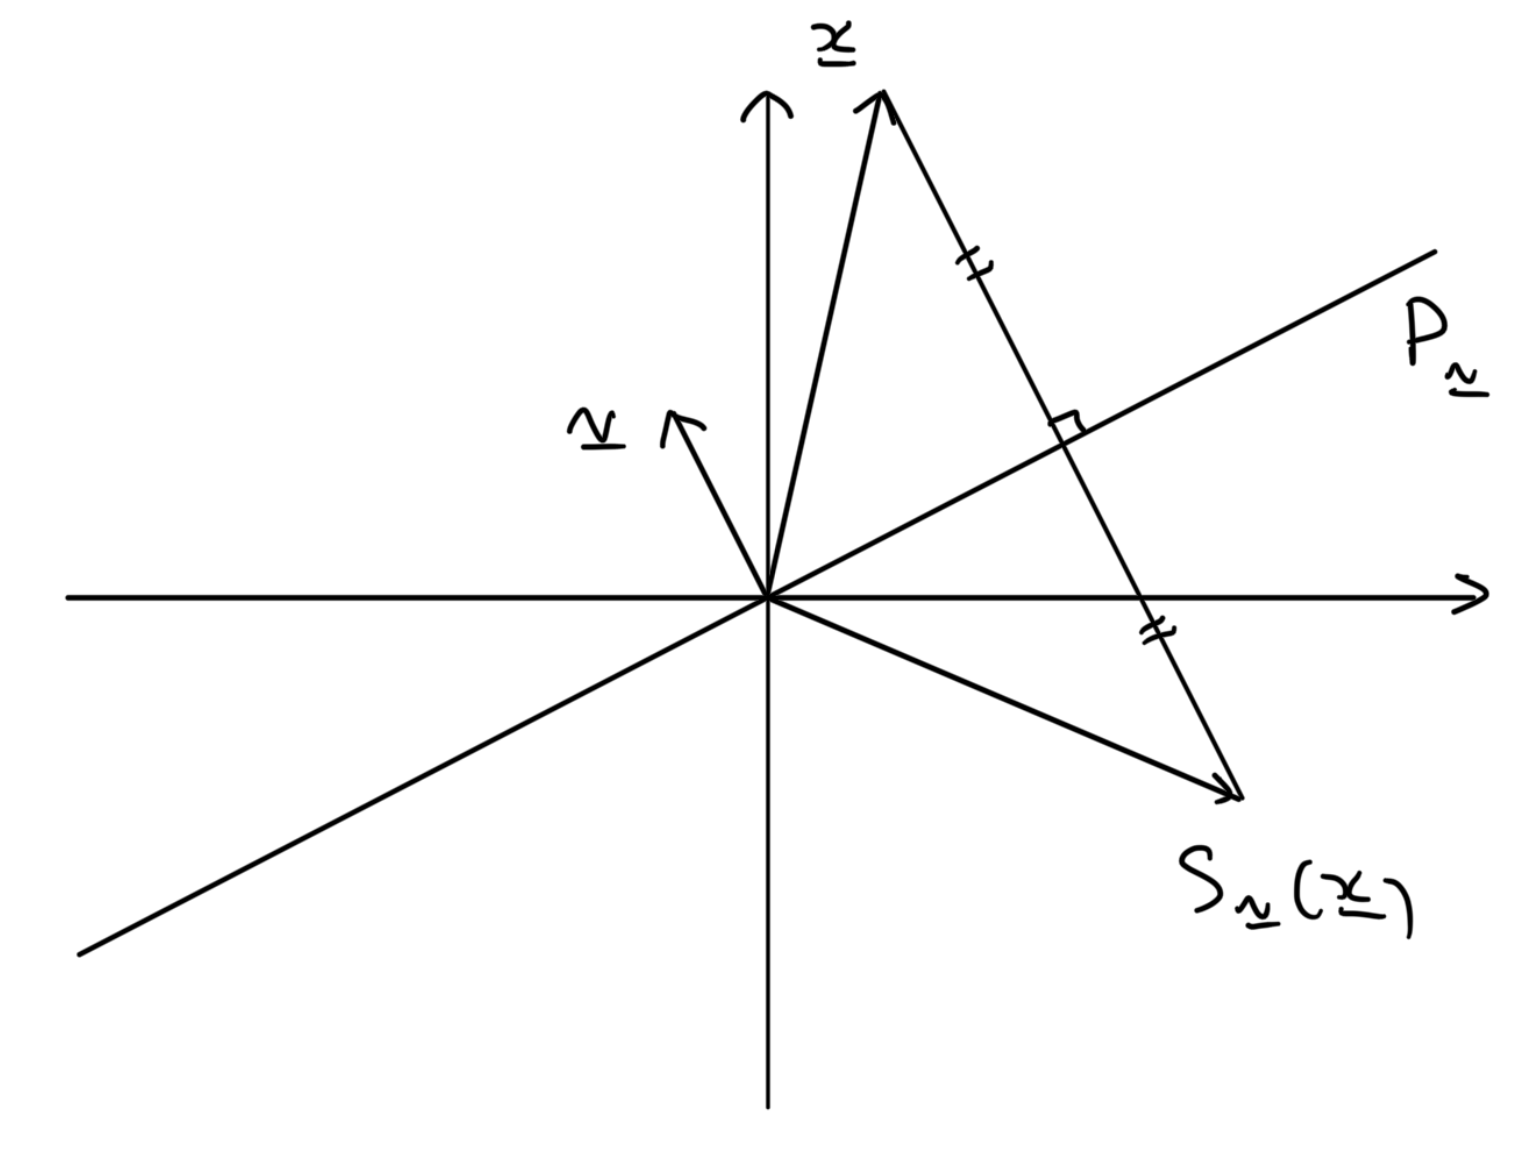
\includegraphics[width=0.8\textwidth]{fig/reflection-in-a-plane.png}
    \caption{Reflection in a Plane}
    \label{fig:reflection-in-plane}
\end{figure}

\begin{remarks}
    \begin{enumerate}
        \item We sometimes use \(S_P\) for the reflection in the plane \(P\).
        \item If we replace \(\vb{v}\) by \(\frac{\vb{v}}{\norm{\vb{v}}}\), and assume \(\norm{\vb{v}} = 1\) (i.e. use the unit vector in \(\vb{v}\) direction, \(\unitv{v}\)), then \(P_{\vb{v}} = P_{\unitv{v}}\), and we have
        \[
        S_{\vb{v}} \pqty{\vb{x}} = \vb{x} - 2 \pqty{\vb{x} \vdot \vb{v}} \vb{v}.
        \]
    \end{enumerate}
\end{remarks}

We study some properties on those reflections.

\begin{lemma}[Reflections are Orthogonal and have Order 2]
    \label{lem:reflections-orthogonal-order-2}%
    For any \(\vb{v} \in \RR^n\setminus\set{\vb{0}}\), we have \(S_{\vb{v}}^2 = I\), and \(S_{\vb{v}} \in \Or\pqty{n}\).
\end{lemma}

\begin{proof}
    Assume \(\norm{\vb{v}} = 1\). Note that \(S_{\vb{v}}\) is indeed linear, so
    \[
        S_{\vb{v}} \in \matrixset_n \pqty{\RR}.
    \]

    For any \(\vb{x} \in \RR^n\), we have
    \begin{align*}
        S_{\vb{v}} \pqty{\vb{x}} \vdot \vb{v} &= \pqty{\vb{x} \vdot \vb{v}} - 2 \pqty{\vb{x} \vdot \vb{v}} \pqty{\vb{v} \vdot \vb{v}} \\
        &= - \pqty{\vb{x} \vdot \vb{v}},
    \end{align*}
    and hence
    \begin{align*}
        S_{\vb{v}}^2 \pqty{\vb{x}} &= S_{\vb{v}} \pqty{\vb{x}} - 2 \pqty{S_{\vb{v}} \pqty{\vb{x}} \vdot \vb{v}} \vb{v} \\
        &= \vb{x} - 2\pqty{\vb{x} \vdot \vb{v}} \vb{v} + 2 \pqty{\vb{x} \vdot \vb{v}} \vb{v} \\
        &= \vb{x},
    \end{align*}
    and hence \(S_{\vb{v}}^2 = I\). Hence, we see \(S_{\vb{v}}\) is non-singular, and hence
    \[
        S_{\vb{v}} \in \GL_n \pqty{\RR}.
    \]

    Finally, we verify that reflections indeed preserve lengths. For any \(\vb{x} \in \RR^n\),
    \begin{align*}
        \norm{S_{\vb{v}} \pqty{\vb{x}}}^2 &= \pqty{\vb{x} - 2 \pqty{\vb{x} \vdot \vb{v}} \vb{v}} \vdot \pqty{\vb{x} - 2 \pqty{\vb{x} \vdot \vb{v}} \vb{v}} \\
        &= \norm{\vb{x}}^2 - 4 \pqty{\vb{x} \vdot \vb{v}}^2 + 4 \pqty{\vb{x} \vdot \vb{v}}^2 \\
        &= \norm{\vb{x}}^2,
    \end{align*}
    and hence \(S_{\vb{v}} \in \Or\pqty{n}\) as desired.
\end{proof}

\begin{remark}
    To see that reflections are in \(\Or\pqty{n} \setminus \SO\pqty{n}\) indeed, let \(\norm{\vb{v}} = 1\), and we pick an orthonormal basis
    \[
        \set{\vb{v}_1, \vb{v}_2, \ldots, \vb{v}_{n - 1}}
    \]
    for the \(\pqty{n-1}\)-dimensional subspace \(P_{\vb{v}}\). Then, in the basis
    \[
        \set{\vb{v}_1, \vb{v}_2, \ldots, \vb{v}_{n - 1}, \vb{v}}
    \]
    for \(\RR^n\), \(S_{\vb{v}}\) is represented by the matrix
    \[
        \pmqty{\dmat{1, 1, \ddots, 1, -1}} = \diag\pqty{1, 1, \ldots, 1, -1}.
    \]

    Therefore, \(\det S_{\vb{v}} = -1\), and \(S_{\vb{v}} \notin \SO\pqty{n}\).
\end{remark}

Reflections are in general not the only elements of \(\Or\pqty{n} \setminus \SO\pqty{n}\), specifically for \(n \geq 3\). A significant reason we study those reflections is they provide a useful generating set for \(\Or\pqty{n}\). Even stronger, we have \autoref{thm:reflections-generate}.

\begin{theorem}[Reflections Generate \(\Or\pqty{n}\)]
    \label{thm:reflections-generate}%
    Every \(A \in \Or\pqty{n}\) is a product of at most \(n\) reflections.
\end{theorem}

\begin{proof}
    We proceed by induction on \(n\).

    \emph{Base Case.} For \(n = 1\), \(\Or\pqty{1} = \set{\pm 1} = \angBrac{S_1} \isomorphic C_2\) and every element is indeed a product of at most \(1\) reflection. Note here \(S_1 \in \Or\pqty{1} \setminus \SO\pqty{1}\) is the reflection in the plane perpendicular to \(\pqty{-1}\), not the trivial group.

    \emph{Induction Step.} Let \(\set{\unitv{e}_1, \unitv{e}_2, \ldots, \unitv{e}_n}\) be the standard basis for \(\RR^n\). If \(A \unitv{e}_n = \unitv{e}_n\), set \(B = A\), so no reflection is needed. Otherwise, let
    \[
        \vb{v} = \unitv{e}_n - A \unitv{e}_n \neq \vb{0}
    \]
    and set \(B = S_{\vb{v}} A\). Then \(B \unitv{e}_n = \unitv{e}_n\), as in \autoref{fig:choice-of-v-for-on}.

    \begin{figure}[ht!]
        \centering
        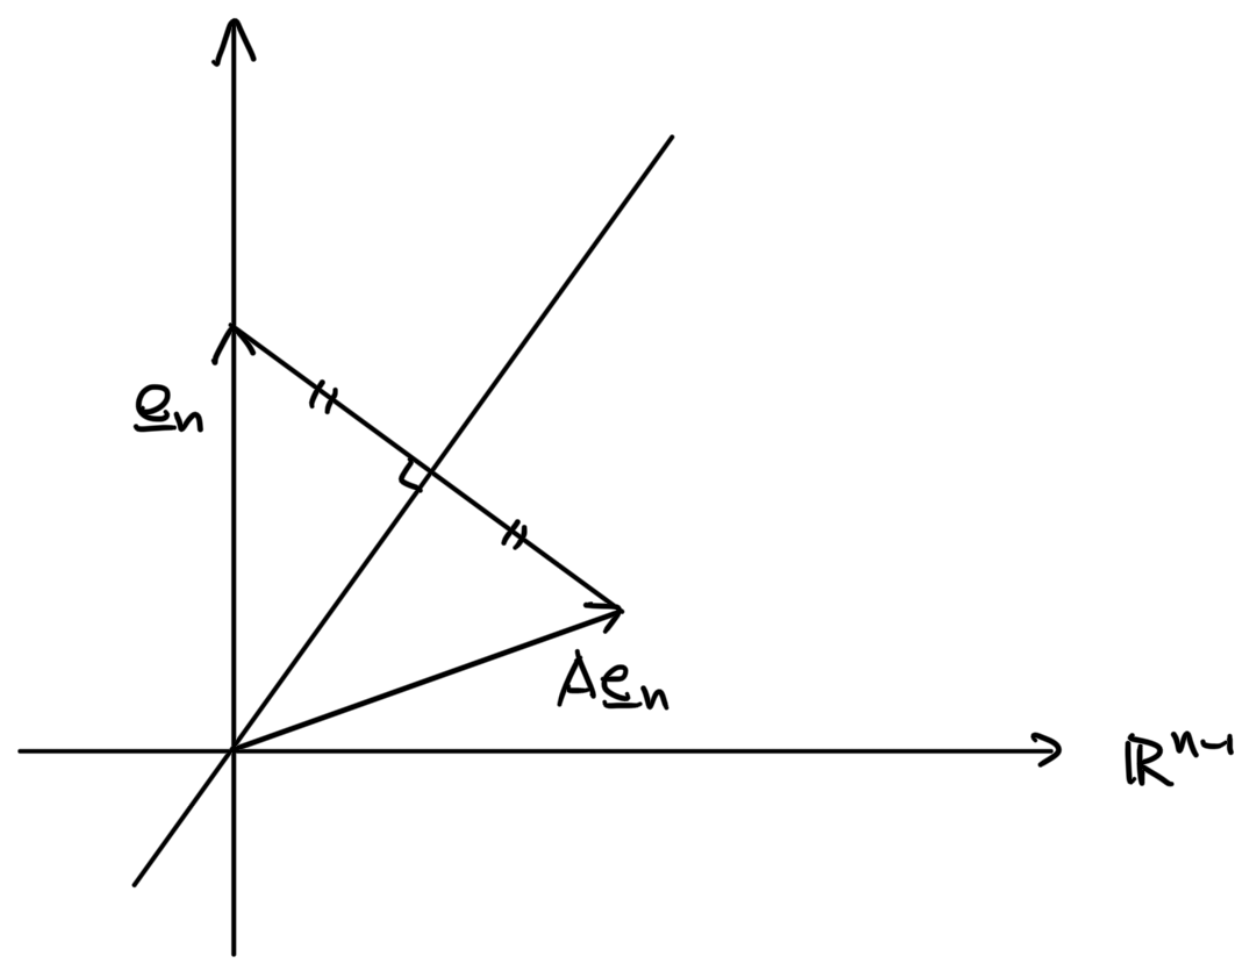
\includegraphics[width=0.6\textwidth]{fig/choice-of-v.png}
        \caption{Choice of \(\vb{v}\) for \(M \in \Or\pqty{n}\)}
        \label{fig:choice-of-v-for-on}
    \end{figure}

    Since \(B\) is orthogonal, \(B\) preserves \(P_{\unitv{e}_n} = \RR^{n - 1} \times \set{\vb{0}}\).

    By induction hypothesis, there exists
    \[
        \vb{v}_1, \vb{v}_2, \ldots, \vb{v}_{n - 1} \in \RR^{n - 1}
    \]
    such that when restricted to \(P_{\unitv{e}_n} = \RR^{n - 1} \times \set{\vb{0}}\),
    \[
        B = S_{\vb{v}_1} S_{\vb{v}_2} \cdots S_{\vb{v}_{n - 1}}
    \]
    and since both sides fix \(\vb{e}_n \notin P_{\unitv{e}_n}\), they agree on the whole of \(\RR^n\) as well. Hence,
    \[
        B = S_{\vb{v}_1} S_{\vb{v}_2} \cdots S_{\vb{v}_{n - 1}}
    \]
    and hence
    \[
        A =
        \begin{cases}
            S_{\vb{v}_1} S_{\vb{v}_2} \cdots S_{\vb{v}_{n - 1}}, & B = A, \\
            S_{\vb{v}} S_{\vb{v}_1} S_{\vb{v}_2} \cdots S_{\vb{v}_{n - 1}}, & B = S_{\vb{v}}A.
        \end{cases}
    \]
\end{proof}

We next aim to characterise elements of \(\Or\pqty{n}\) and \(\SO\pqty{n}\) in lower dimensions, specifically for \(\Or\pqty{2}\), \(\SO\pqty{2}\) and \(\SO\pqty{3}\).

\begin{lemma}[Elements in \(\Or\pqty{2}\)]
    \label{lem:elements-in-o2}%
    Let \(M \in \Or\pqty{2}\).
    \begin{enumerate}
        \item If \(M \notin \SO\pqty{2}\), then \(M\) is a reflection.
        \item If \(M \in \SO\pqty{2}\), then \(M\) is a rotation about \(O\).
    \end{enumerate}
\end{lemma}

\begin{proof}
    Recall that \(\det S_{\vb{v}} = -1\), so
    \[
        \det \pqty{S_{\vb{v}_1} S_{\vb{v}_2} \cdots S_{\vb{v}_k}} = \pqty{-1}^k.
    \]

    By \autoref{thm:reflections-generate}, we may take \(k \leq 2\).
    \begin{enumerate}
        \item If \(M \notin \SO\pqty{2}\), then \(k\) is odd, and hence \(k = 1\) giving \(M\) is a reflection.
        \item If \(M \in \SO\pqty{2}\), then \(k\) is even, so unless \(M = I\), then 
        \[
            M = S_{\vb{u}} S_{\vb{v}}
        \]
        for some \(\vb{u}, \vb{v} \in \RR^2\) not parallel.

        Now we claim that \(M\) only fixes the origin and hence is a rotation. Suppose for contradiction, that for some \(\vb{x} \neq \vb{0}\), we have that \(M\) fixes \(\vb{x}\), note that
        \[
            S_{\vb{u}} S_{\vb{v}} \vb{x} = \vb{x} \iff S_{\vb{u}} \vb{x} = S_{\vb{v}} \vb{x}.
        \]

        \(\vb{v}\) is parallel to \(\vb{x} - S_{\vb{v}} \vb{x}\), and \(\vb{u}\) is parallel to \(\vb{x} - S_{\vb{u}} \vb{x}\). But since \(\vb{x} \neq \vb{0}\), we have \(\vb{x} \neq S_{\vb{v}} \vb{x} = S_{\vb{u}} \vb{x}\), and hence \(\vb{u}\) is parallel to \(\vb{v}\), which is not possible.

        Therefore, \(M\) only fixes the origin \(O\), as desired.
    \end{enumerate}
\end{proof}

\begin{remark}
    Let \(M \in \SO\pqty{2}\), since the columns form an orthonormal basis, we have
    \[
        M = \pmqty{a & b \\ -b & a}
    \]
    with \(a, b \in \RR\) and \(a^2 + b^2 = \det M = 1\). Then, let \(a = \cos \theta, b = \sin \theta\) for some \(\theta \in \RR\), and hence we have
    \[
        M = \pmqty{\cos \theta & \sin \theta \\ - \sin \theta & \cos \theta}.
    \]

    Similarly, if \(M \in \Or\pqty{2} \setminus \SO\pqty{2}\) is some reflection, we have
    \[
        M = \pmqty{a & b \\ b & -a}
    \]
    with \(a, b \in \RR\) and \(-a^2 - b^2 = \det M = -1\). Then, let \(a = \cos \theta, b = \sin \theta\) for some \(\theta \in \RR\), and hence we have
    \[
        M = \pmqty{\cos \theta & \sin \theta \\ \sin \theta & -\cos \theta}.
    \]
\end{remark}

\begin{lemma}[Elements in \(\SO\pqty{3}\)]
    \label{lem:elements-in-so3}%
    If \(M \in \SO\pqty{3}\), then \(M\) is a rotation.
\end{lemma}

\begin{proof}
    Similarly to the proof of \autoref{lem:elements-in-o2}, \(M\) is a product of at most \(3\) reflections. So either \(M = I\), or \(M = S_{\vb{u}} S_{\vb{v}}\) for some non-parallel \(\vb{u}, \vb{v} \in \RR^3\).

    Since \(n = 3\), we have
    \[
        P_{\vb{u}} \cap P_{\vb{v}} = l
    \]
    for a line \(l\), so \(M\) fixes \(l\).

    Also, proceeding similarly as in \autoref{lem:elements-in-o2} shows us either \(S_{\vb{u}} = S_{\vb{v}}\) giving \(M = I\) or the fixed point is in \(P_{\vb{u}} \cap P_{\vb{v}} = l\).

    Therefore, any non-trivial \(M\) only fixes a line \(l\), hence a rotation.
\end{proof}